\documentclass{article}

% if you need to pass options to natbib, use, e.g.:
% \PassOptionsToPackage{numbers, compress}{natbib}
% before loading nips_2018

% ready for submission
\usepackage{nips_2018}

% to compile a preprint version, e.g., for submission to arXiv, add
% add the [preprint] option:
% \usepackage[preprint]{nips_2018}

% to compile a camera-ready version, add the [final] option, e.g.:
% \usepackage[final]{nips_2018}

% to avoid loading the natbib package, add option nonatbib:
% \usepackage[nonatbib]{nips_2018}

\usepackage[utf8]{inputenc} % allow utf-8 input
\usepackage[T1]{fontenc}    % use 8-bit T1 fonts
\usepackage{hyperref}       % hyperlinks
\usepackage{url}            % simple URL typesetting
\usepackage{booktabs}       % professional-quality tables
\usepackage{amsfonts}       % blackboard math symbols
\usepackage{nicefrac}       % compact symbols for 1/2, etc.
\usepackage{microtype}      % microtypography


% The \author macro works with any number of authors. There are two
% commands used to separate the names and addresses of multiple
% authors: \And and \AND.
%
% Using \And between authors leaves it to LaTeX to determine where to
% break the lines. Using \AND forces a line break at that point. So,
% if LaTeX puts 3 of 4 authors names on the first line, and the last
% on the second line, try using \AND instead of \And before the third
% author name.
\usepackage{amssymb}
\usepackage{amsmath,amsthm}
\usepackage{float}
\usepackage{url}
\usepackage{setspace}
\usepackage{hyperref}
\usepackage{todonotes}
\usepackage{amsthm} 
\usepackage[ruled,vlined,linesnumbered]{algorithm2e} 
\usepackage{makecell}
\usepackage{upgreek}
\onehalfspacing
\usepackage{pdfpages}
\usepackage{times}
\usepackage{multirow}
\usepackage[toc,page]{appendix}
\usepackage{listings}
\newtheorem{thm}{Theorem}
\newtheorem{lemma}[thm]{Lemma}
\newtheorem{definition}[thm]{Definition}
\newtheorem{observation}[thm]{Observation}
\newtheorem{theorem}[thm]{Theorem}
\newtheorem{claim}[thm]{Claim}
\newtheorem{example}[thm]{Example}
\newtheorem{proposition}[thm]{Proposition}
\usepackage{color,soul}
\usepackage{tikz}
\usetikzlibrary{arrows,shapes.geometric,shapes.arrows}
\usepackage{pgfplots}
\usepackage{multirow}


\DeclareMathOperator{\supp}{support}
\DeclareMathOperator{\support}{support}
\DeclareMathOperator{\Trim}{Trim}
\DeclareMathOperator{\LTrim}{LTrim}
\SetKwFunction{mEqOne}{mEqOne} 
\DeclareMathOperator{\KlmApprox}{KolmogorovApprox}
\DeclareMathOperator{\OptTrim}{KolmogorovApprox}
\title{Kolmogorov Approximation}



\begin{document}
% \nipsfinalcopy is no longer used

\maketitle


\begin{definition}
A random variable $X'$ is an $m$-optimal-approximation of a random variable $X$ if $|\support(X')| \leq m$ and there is no random variable $X''$ such that $|\support(X'')| \leq m$ and $d_k(X,X'') < d_k(X,X')$.
\end{definition}

\begin{lemma}
	For any discrete random variable $X$ and any $m \in \mathbb{N}$, there is an $m$-optimal-approximation $X'$ of $X$ such that $\support(X') \subseteq \support(X)$.
\end{lemma}
\begin{proof}
Assume there is a random variable $X''$ with support size $m$ such that $d_K(X,X'')$ is minimal but $\support(X'')\nsubseteq\support(X)$.
We will show how to transform $X''$ support such that it will be contained in $\support(X)$. Let $v'$ be the first $v'\in\support(X'')$ and $v' \not\in\support(X)$. Let $v=\max\{i: i<v' \wedge i\in\support(X)\}$. Every $v'$ we will replace with $v$ and name the new random variable $X'$, we will show that $d_K(X,X'') = d_K(X,X')$. First, note that:
$F_{X''}(v')=F_{X'}(v)$, $F_{X}(v')=F_{X}(v)$.
Second,  $F_{X'}(v')-F_{X}(v') = F_{X'}(v)-F_{X}(v)$. Therefore, $d_K(X,X'') = d_K(X,X')$ and $X'$ is also an optimal approximation of $X$.
\end{proof}

\begin{observation}\label{obs:ab}
	$max\{|a|,|b|\} \geq |a-b|/2$
\end{observation}
\begin{proof}
	By the triangle inequality, the sum of $|a|$ and $|b|$ is greater or equal to $|a-b|$, thus one of them must be larger or equal to half of it. 
%Assume by contradiction that $max\{|a|,|b|\} < 1/2|a-b|$ and assume without loss of generality that $|a|>|b|$. We get that $2|a|<|a-b|$ which is possible if and only if $|a|<|b|$, in contradiction to that $|a|>|b|$.
\end{proof}

\begin{lemma}\label{lem:geq}
	For $x_1, x_2 \in \support(X) \cup \{-\infty,\infty\}$ such that $x_1 < x_2$, if $P(x_1 < X' < x_2)=0$  then 
	$d_k(X,X') \geq P(x_1 < X < x_2)/2$.
\end{lemma}
\begin{proof}
	Let $\hat x=\max \{x \in \support(X) \cap\{ -\infty, \infty\}  \colon x < x_2 \}$. By definition, $d_k(X,X') \geq \max \{|F_X(x_1) - F_X'(x_1)|, |F_X(\hat x) - F_X'(\hat x)| \}$. From Observation~\ref{obs:ab}, $d_k(X,X') \geq 1/2|F_X(x_1) - F_X(\hat x) + F_X'(x_1)- F_X'(\hat x)|$. Since it is given that $P(x_1 < X' < x_2)=0$, $d_k(X,X') \geq 1/2|F_X(x_1) - F_X(\hat x) | =  P(x_1 < X \leq \hat x)/2 = P(x_1 < X < x_2)/2$.
\end{proof}


\begin{lemma}\label{lem:geq2}
	For $x_1, x_2 \in \support(X) \cup \{-\infty,\infty\}$ such that $x_1=-\infty$ or  $x_2=\infty$, if $P(x_1 < X' < x_2)=0$  then 
	$d_k(X,X') \geq P(x_1 < X < x_2)$.
\end{lemma}
\begin{proof}
	Let $\hat x=\max \{x \in \support(X) \cap\{ -\infty, \infty\}  \colon x < x_2 \}$. By definition $d_k(X,X') \geq \max \{|F_X(x_1) - F_X'(x_1)|, |F_X(\hat x) - F_X'(\hat x)| \}$. If $x_1=-\infty$ then $d_k(X,X') \geq \{|F_X(\hat x) - F_X'(\hat x)| \}$ since $F_X(-\infty) = F_X'(-\infty) = 0$. Furthermore, $F_X'(\hat x) = 0$ since it is given that $P(x_1 < X' < x_2)=0$. Therefore we get that $d_k(X,X') \geq F_X(\hat x) = P(x_1 < X \leq \hat x) = P(x_1 < X \leq x_2)$. 
	If $x_1=\infty$ then $d_k(X,X') \geq \{|F_X(x_1) - F_X'(x_1)| \}$ since $F_X(\infty) = F_X'(\infty) = 1$. Furthermore, $F_X'(x_1) = 1$ since it is given that $P(x_1 < X' < x_2)=0$. Therefore we get that $d_k(X,X') \geq |F_X(x_1)-1| = |1-F_X(\hat x)-| = P(x_1 < X \leq \hat x) = P(x_1 < X < x_2)$.
\end{proof}


\begin{definition} Let:
	\[
	w(x_1,x_2)=
	\begin{cases}
		P(x_1 < X < x_2) & \text{if $x_1=-\infty$ or $x_2 = \infty$;} \\
		P(x_1 < X < x_2)/2 & \text{otherwise.} \\	
	\end{cases}
	\]
\end{definition} 


\begin{claim}
	For a random variable $X$, an ordered set $S=\{x_1<\dots<x_m\} \subset \support(X)$, $x_0=-\infty$ and $x_{n+1}=\infty$, there is no random variable $X'$ such that $\support(X')=S$ and $d_k(X,X') < \max\limits_{i=0,\dots,m} w(x_{i}, x_{i+1})$.
\end{claim}
\begin{proof}
	Let $i$ be the index that maximizes $w(x_{i}, x_{i+1})$. If $0<i<n-1$ then $d_k(X,X') \geq w(x_{i}, x_{i+1})$ by Lemma~\ref{lem:geq}. If $i=0$ or $i=n+1$ the same follows from Lemma~\ref{lem:geq2}.
\end{proof}


\begin{claim}
	For a random variable $X$, an ordered set $S=\{x_1<\dots<x_m\} \subset \support(X)$, $x_0=-\infty$ and $x_{m+1}=\infty$, there is a random variable $X'$ such that $\support(X')=S$ and $d_k(X,X')= \max\limits_{i=0,\dots,m} w(x_{i}, x_{i+1})$.
\end{claim}
\begin{proof}
Define $X'$ by $f_{X'}(x_i) = w(x_{i-1},x_i) + w(x_i,x_{i+1}) + f_{X}(x_i)$ for $i=1,\dots,m$ and $f_{X'}(x)=0$ for $x \notin S$.
\end{proof}

\begin{definition}\label{def:RVpartition}
	We say that a random variable $X'$ is a \emph{consecutive approximation} of a random variable $X$ if there is a consecutive partition $P=\{B_1,\dots,B_n\}$ of $\support(X)$ such that the probability mass function (PMF) of $X'$ is 
	$$f_{X'}(t) = 
	\begin{cases} 
	Pr(X {\in} B_i) &  \text{if $t = \min(B_i)$ for some $i$;}\\
	0          &  \text{otherwise.}
	\end{cases}$$
\end{definition}



Chakravarty, Orlin, and Rothblum~\cite{chakravarty1982partitioning} proposed a polynomial-time method that, given certain objective functions (additive), finds an optimal consecutive partition. Their method involves the construction of a graph such that the (consecutive) set partitioning problem is reduced to the problem of finding the shortest path in that graph.

The $\KlmApprox$ algorithm (Algorithm~\ref{alg:optapprox}) starts by constructing a directed weighted graph $G$ similar to the method of Chakravarty, Orlin, and Rothblum~\cite{chakravarty1982partitioning}. The nodes $V$ consist of the support of $X$ together with an extra two nodes $\infty$ and $-\infty$ for technical reasons, whereas the edges $E$ connect every pair of nodes in one direction (lines 1-2). The weight $w$ of each edge $e=(i,j)\in E$ is determined by on of two cases. The first is where $i$ or $j$ are the source or target nodes respectively. In this case the weight is the probability of $X$ to get a value between $i$ and $j$, non inclusive, i.e., $w(e)=Pr(i<X<j)$ (lines 4-5). The second case is where $i$ or $j$ are not a source or target nodes, here the weight is the probability of $X$ to get a value between $i$ and $j$, non inclusive, divided by two i.e., $w(e)=Pr(i<X<j)/2$ (lines 6-7). The values taken are non inclusive, since we are interested only in the error value.
The source node of the shortest path problem at hand corresponds to the $-\infty$ node added to $G$ in the construction phase, and the target node is the extra node $\infty$.
The set of all solution paths in $G$, i.e., those starting at $-\infty$ and ending in $\infty$ with at most $m$ edges, is called $paths(G)$. The goal is to find the path $l^*$ in $paths(G)$ with the lightest bottleneck (lines 8-9). This can be achieved by using the $Bellman-Ford$ algorithm with two tweaks. The first is to iterate the graph $G$ in order to find only paths with length of at most $m$ edges. The second is to find the lightest bottleneck as opposed to the traditional objective of finding the shortest path. This is performed by modifying the manner of ``relaxation'' to $bottleneck(x) = min[max(bottleneck(v),w(e))]$, done also in~\cite{shufan2011two}. Consequently, we find the lightest maximal edge in a path of length $\leq m$, which represents the minimal error, $\varepsilon^*$, \hl{defined in Definition}~\ref{def:optimalapprox}. $X'$ is then derived from the resulting path $l^*$ (lines 10-17). Every node $n \in l^*$ represent a value in the new calculated random variable $X'$, we than iterate the path $l^*$ to fine the probability of the event $f_{X'}(n)$. For every edge $(i,j)\in l^*$ we determine: if $(i,j)$ is the first edge in the path $ l^*$ (i.e.  $i==-\infty$), then node $j$ gets the full weight $w(i,j)$ and it's own weight in $X$ such that $f_{X'}(j) = f_{X}(j) +  w(i,j)$ (lines 11-12). If $(i,j)$ in not the first nor the last edge in path $l^*$ then we divide it's weight between nodes $i$ and $j$ in addition to their own original weight in $X$ and the probability that already accumulated (lines 16-17). If $(i,j)$ is the last edge in the path $ l^*$ (i.e.  $i==\infty$) then node $i$ gets the full weight $w(i,j)$ in addition to what was already accumulated such that $f_{X'}(j) = f_{X'}(j) +  w(i,j)$ (lines 13-14).


\begin{algorithm}\label{alg:optapprox}
	\DontPrintSemicolon
	\SetKwFunction{Convolv}{Conv}
	\SetKwFunction{getPartition}{getPartition}
	\SetKwFunction{bellmanFordMinMaxM}{bellmanFordMinMaxM}
	$S = \support(X)\cup \{\infty,-\infty\}$\;
	$G=(V,E)=(S, \{ (x_i,x_j) \in S^2 \colon  j>i \})$ \;
	
	\ForEach{$e=(i,j) \in  E $ }{
		\If {$i=\infty \text{ OR } j=-\infty$}{
			$w(e) = Pr(i<X<j)$
		}
		\Else{$w(e) = Pr(i<X<j)/2$}
	}
	
	/* The following can be obtained, e.g., using the Bellman-Ford algorithm */\;
	$l^*= \operatorname{argmin}\limits_{l \in paths(G),|l|\leq m}  \max \{ w(e)\colon e \in l  \}$ \;
	
	\ForEach{$e=(i,j) \in  l^* $ }{
		\If {$i=-\infty$}{
			$f_{X'}(j) = f_{X}(j) + Pr(i\leq X<j)$
		}
		\ElseIf{$j==\infty$}{
			$f_{X'}(i) = f_{X'}(i) + Pr(i\leq X<j)$
		}
		\Else{
			$f_{X'}(i) = f_{X'}(i) + Pr(i\leq X<j)/2$\;
			$f_{X'}(j) = f_{X}(j) + Pr(i\leq X<j)/2$\;
		}
		
	}	
	\Return $X'$\;
	
	\caption{$\KlmApprox (X, m)$}  
	\label{alg:sequence}
\end{algorithm}

\begin{theorem}\label{the:complexity}
	The $\KlmApprox(X,m)$ algorithm runs in time $O(mn^2)$, using $O(n^2)$ memory where $n=|\support(X)|$.
\end{theorem}

\begin{proof}
	Constructing the graph $G$ takes $O(n^2)$. The number of edges is $O(E)\approx O(n^2)$ and for every edge the weight is at most the sum of all probabilities between the source node $-\infty$ and the target node $\infty$, which can be done efficiently by aggregating the weights of already calculated edges. 
	The construction is also the only stage that requires memory allocation, specifically $O(E+V)=O(n^2)$.
	Finding the shortest path takes $O(m(E+V))\approx O(mn^2)$. Since $G$ id DAG (directed acyclic graph) finding shortest path takes $O(E+V)$. We only need to find paths of length $\leq m$, which takes $O(m(E+V))$.
	Deriving the new random variable $X'$ from the computed path $l^*$ takes $O(mn)$. For every node in $l^*$ (at most $m$ nodes), calculating the probability $P(s<X<\infty)$ takes at most $n$. 
	To conclude, the worst case run-time complexity is $O(n^2+mn^2+mn)=O(mn^2)$ and memory complexity is $O(E+V)=O(n^2)$.
\end{proof}

\begin{example}\textbf{Why one sided Kolmogorov approximation in not sufficient in this case?}
	Consider the following random variable $X$: 
	$$
	f_{X}(t) = \begin{cases}
	1/3           & \text{if $t=1$ or $t=2$} ;  \\ 
	1/6           & \text{if $t=3$ or $t=4$};  \\  
	0             & \text{otherwise.}
	\end{cases}
	$$
	
	There are various partitioned random variables of size $m=2$ which provide some approximation in regards to Kolmogorov distance, some are presented as follows:
	$$
	f_{X'_1}(t) = \begin{cases}
	2/3           & \text{if } t=1;  \\ 
	1/3           & \text{if } t=3;  \\  
	0             & \text{otherwise.}
	\end{cases}
	$$
	In this case $d_K(X, X'_1) = 1/3$.
	
	$$
	f_{X'_2}(t) = \begin{cases}
	1/3           & \text{if } t=1;  \\ 
	2/3           & \text{if } t=2;  \\  
	0             & \text{otherwise.}
	\end{cases}
	$$
	In this case $d_K(X, X'_2) = 1/3$.
	
	$$
	f_{X'_3}(t) = \begin{cases}
	2/3           & \text{if } t=2;  \\ 
	1/3           & \text{if } t=3;  \\  
	0             & \text{otherwise.}
	\end{cases}
	$$
	In this case $d_K(X, X'_3) = 1/3$.
	
	However, none of the above random variables provides an optimal approximation. Here is an optimal approximation which can not be achieved by a regular partitioned random variable:
	
	$$ 	f_{X''}(t) = \begin{cases}
	1/2           & \text{if } t=1;  \\ 
	1/2           & \text{if } t=3;  \\  
	0             & \text{otherwise.}
	\end{cases}
	$$
	In this case $d_K(X, X'') = 1/6$.
\end{example}

\subsection{Experiments and Results}
In the first experiment we focus on the problem of task trees with deadlines, and consider three types of task trees.
The first type includes logistic problems of transporting packages by trucks and airplanes (from IPC2 http://ipc.icaps-conference.org/). Hierarchical plans of those logistic problems were generated by the JSHOP2 planner \cite{nau2003shop2} (see example problem, Figure~\ref{fig:logistics}). 
The second type consists of task trees used as execution plans for the ROBIL team entry in the DARPA robotics challenge (DRC simulation phase), and the third type is of linear plans (sequential task trees).
The primitive tasks in all the trees are modeled as discrete random variables with support of size $M$ obtained by discretization of uniform distributions over various intervals. The number of tasks in a tree is denoted by $N$. 

We fed the approximation algorithm for solving the deadline problem with two different methods of the one-sided Kolmogorov approximation -- the $\OptTrim$ and the $\Trim$ operators. 
The parameter $m$ of $\OptTrim$ corresponds to the inverse of $\varepsilon$ given to the $\Trim$ operator. Note that in order to obtain some error $\varepsilon$, one must take into consideration the size of the task tree, $N$, therefore, $m/N=1/(\varepsilon\cdot N)$ (see Lemma~\ref{errorM} and Theorem~\ref{trimtoopttrim}). We ran the exact algorithm as reference, the approximation algorithm using $\OptTrim$ as its operator with $m=10\cdot N$, the approximation algorithm using the $\Trim$ operator with $\varepsilon={0.1/N}$, and two simple simulations, with a different samples number $s=10^4$ and $s=10^6$. 
\begin{table}[th]
	\scriptsize
	\centering
	\begin{tabular}{|c|c|c|c|c|c|}
		\hline
		\multirow{2}{*}{Task Tree} & \multirow{2}{*}{$M$} & {$\OptTrim$} & {$\Trim$} & \multicolumn{2}{c|}{Sampling} \\ \cline{3-6} 
		&	& $m/N{=}10$  & $\varepsilon\cdot N{=}0.1$ & $s{=}10^{4}$& $s{=}10^{6}$ \\ \hline
		\hline
		
		%N=34
		
		\multirow{2}{*}{Logistics} & 2& 0 &  0.0019 &  0.007 & 0.0009  \\ \Xcline{2-6}{1pt}
		{\tiny $(N=34)$}& 4& 0.0046&  0.0068  &   0.0057 & 0.0005 \\\Xhline{1pt}
		
		%N=45
		\multirow{2}{*}{Logistics}  & {2} & 0.0005 &  0.002 &  0.015& 0.001
		\\ \Xcline{2-6}{1pt} 
		{\tiny $(N{=}45)$} & {4} & 0.003 & 0.004 & 0.008 & 0.0006  
		\\\Xhline{1pt}
		
		%N=47
		\multirow{2}{*}{DRC-Drive}  
		&2	&	0.004&  0.009  & 0.0072 & 0.0009  \\ \Xcline{2-6}{1pt}
		
		{\tiny $(N{=}47)$}& {4}& 0.008&  0.019   & 0.0075  & 0.0011 \\  \Xhline{1pt}
		
		
		%N=10
		\multirow{2}{*}{Sequential}  & {4} & 0.024 &  0.04 & 0.008 & 0.0016 \\ \Xcline{2-6}{1pt}  
		
		{\tiny $(N{=}10)$} & {10} & 0.028  &  0.06  & 0.0117  & 0.001 \\\Xhline{1pt}
		
		
		
	\end{tabular}
	\caption{Comparison of estimation errors with respect to the reference exact computation on various task trees.}
	\label{tab:errors}
	
\end{table}

Table~\ref{tab:errors} shows the results of the main experiment. The quality of the solutions provided by using the $\OptTrim$ operator are better (lower errors) than those provided by the $\Trim$ operator, following the optimality guarantees, but is interesting to see that the quality gaps happen in practice in each of the examined task trees. However, in some of the task trees the sampling method produced better results than the approximation algorithm with $\OptTrim$. Nevertheless, the approximation algorithm comes with an inherent advantage of providing an exact quality guarantees, as opposed to the probabilistic guarantees provided by sampling.

In order to better understand the quality gaps in practice between $\OptTrim$ and $\Trim$, we investigate their relative errors when applied on single random variables with different sizes of the support ($M$), and different support sizes of the resulting random variable approximation ($m$). In each instance of this experiment, a random variable is randomly generated by choosing the probabilities of each element in the support from a uniform distribution and then normalizing these probabilities so that they sum to one.

Tables~\ref{tab:trimvsoptrim} and~\ref{tab:trimvsoptrim2} present the error produced by $\OptTrim$ and $\Trim$ on random variables with supports sizes of $M=100$ and $M=1000$, respectively. The depicted results in these tables are averages over several instances of random variables for each entry (50 instances in Table~\ref{tab:trimvsoptrim} and 10 instances in Table~\ref{tab:trimvsoptrim2}). The two central columns in each table show the average error of each method, whereas the right column presents the average percentage of the relative error of the $\Trim$ operator with respect to the error of the optimal approximation provided by $\OptTrim$; the relative error of each instance is calculated by $(\Trim/\OptTrim)-1$. According to the depicted results it is evident that increasing the support size of the approximation $m$ reduces the error, as expected, in both methods. However, the interesting phenomenon is that the relative error percentage of $\Trim$ grows with the increase of $m$.

\begin{table}[tbp]
	\scriptsize
	\centering
	\begin{tabular}{|c|c|c|c|}
		\hline
		m  & $\OptTrim$	& $\Trim$	& Relative error  \\ \hline
		2  & 0.491			& 0.493		& 0.4\%            \\ \hline
		4  & 0.242			& 0.247 	& 2.1\%            \\ \hline
		8  & 0.118 			& 0.123 	& 4.4\%            \\ \hline
		10 & 0.093			& 0.099		& 6\%              \\ \hline
		20 & 0.043			& 0.049		& 15\%             \\ \hline
		50 & 0.013 			& 0.019 	& 45.4\%           \\ \hline
	\end{tabular}
	\caption{$\OptTrim$ vs. $\Trim$ on randomly generated random variables with original support size $M=100$.}
	\label{tab:trimvsoptrim}
\end{table}



\begin{table}[tbp]
	\scriptsize
	\centering
	\begin{tabular}{|c|c|c|c|}
		\hline
		m   & $\OptTrim$	& $\Trim$	& Relative error  \\ \hline
		50  & 0.0193			& 0.0199	& 3.4\%            \\ \hline
		100 & 0.0093			& 0.0099	& 7.1\%            \\ \hline
		200 & 0.0043			& 0.0049	& 15.7\%           \\ \hline
	\end{tabular}
	\caption{$\OptTrim$ vs. $\Trim$ on randomly generated random variables with original support size $M=1000$.}
	\label{tab:trimvsoptrim2}
\end{table}

The above experiments display the quality of approximation provided by the $\OptTrim$ algorithm, but it comes with a price tag in the form of run-time performance. The time complexity of both the $\Trim$ operator and the sampling method is linear in the number of variables, resulting in much faster run-time performances than $\OptTrim$, for which the time complexity is only polynomial (Theorem~\ref{the:complexity}), not linear. The run-time of the exact computation, however,  may grow exponentially. Therefore, we examine in the next experiment the problem sizes in which it becomes beneficial in terms of run-time to use the proposed approximation.

Figure~\ref{fig:runtime} presents a comparison of the run-time performances of an exact computation and approximated computations with $\OptTrim$ and $\Trim$ as operators. The computation is a summation of a sequence of random variables with support size of $M{=}10$, where the number $N$ of variables varies from 6 to 19. In this experiment, we executed the $\OptTrim$ operator with $m{=}10$ after performing each convolution between two random variables, in order to maintain a support size of 10 in all intermediate computations. 
Equivalently, we executed the $\Trim$ operator with $\varepsilon=0.1$.
The results clearly show the exponential run-time of the exact computation, caused by the convolution between two consecutive random variables. In fact, in the experiment with $N{=}20$, the exact computation ran out of memory. These results illuminate the advantage of the proposed $\OptTrim$ algorithm that balances between solution quality and run-time performance -- while there exist other, faster, methods (e.g., $\Trim$), $\OptTrim$ provides high-quality solutions in reasonable (polynomial) time, which is especially important when an exact computation is not feasible, due to time or memory.

\begin{figure}[htb]
	\scriptsize	
	\centering 
	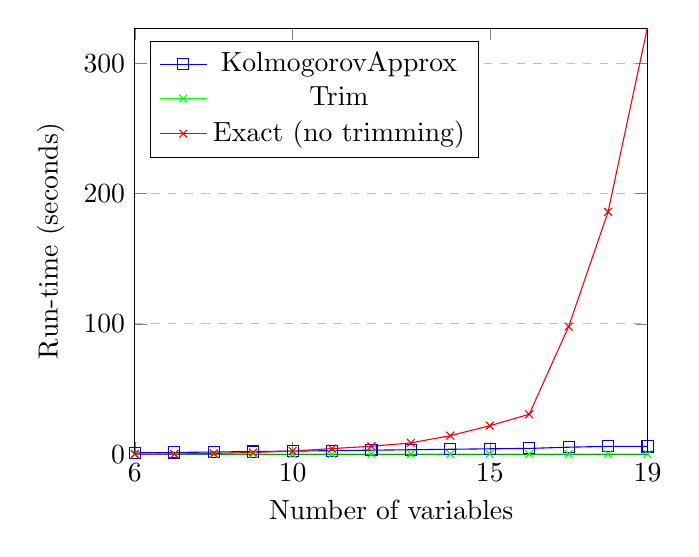
\begin{tikzpicture}
	\begin{axis}[
	scale=.95,
	xlabel={Number of variables},
	ylabel={Run-time (seconds)},
	xmin=6, xmax=19,
	ymin=0, ymax=327,
	xtick={6,10,15,19},
	legend pos=north west,
	ymajorgrids=true,
	grid style=dashed,
	]
	
	\addplot[
	color=blue,
	mark=square,
	]
	coordinates { 
		(6 , 0.967791080475) 
		(7 , 1.26214194298) 
		(8 , 1.60830593109) 
		(9 , 1.97642302513) 
		(10, 2.28711390495) 
		(11, 2.67097711563) 
		(12, 3.01373195648) 
		(13, 3.3420279026) 
		(14, 3.71830201149) 
		(15, 4.08019995689) 
		(16, 4.3857190609) 
		(17, 5.30444002151)
		(18, 5.97745299339) 
		(19, 5.91222810745) 
	};
	\addlegendentry{$\OptTrim$}
	
	\addplot[
	color=green,
	mark=x,
	]
	coordinates {
		(6  , 0.000465154647827)
		(7  , 0.000580787658691)
		(8  , 0.000672817230225)
		(9  , 0.000787973403931)
		(10 , 0.000914096832275)
		(11 , 0.00101804733276)
		(12 , 0.00112104415894)
		(13 , 0.0012149810791)
		(14 , 0.00134491920471)
		(15 , 0.00143694877625)
		(16 , 0.00155091285706)
		(17 , 0.00166893005371)
		(18 , 0.00178194046021)
		(19 , 0.00198793411255)
	};
	\addlegendentry{$\Trim$}
	
	\addplot[
	color=red,
	mark=x,
	]
	coordinates {
		(6  , 0.00977492332458)
		(7  , 0.0880949497223)
		(8  , 0.556006193161)
		(9  , 1.23386096954)
		(10 , 2.37807798386)
		(11 , 4.2376730442)
		(12 , 6.03167200089)
		(13 , 8.61568593979)
		(14 , 14.1664741039)
		(15 , 21.7874569893)
		(16 , 30.5902190208)
		(17 , 97.9485061169)
		(18, 186.025614977) 
		(19, 327.884781122) 
	};
	\addlegendentry{Exact (no trimming)}
	
	\end{axis}
	\end{tikzpicture}
	\caption{Run-time of a long computation with $\OptTrim$, with $\Trim$, and without any trimming (exact computation).}
	\label{fig:runtime}
\end{figure}

\bibliography{library,Trim_Optimum}{}
\bibliographystyle{apalike}

\end{document}

